% !TeX spellcheck = en_US
%!TEX TS-program = xelatex  
%!TEX encoding = UTF-8 Unicode

\documentclass[AcMaster]{ref/BJTU-thesis}  %硕士
%\documentclass[Doctor]{ref/BJTU-thesis}	%博士
%%%%%%%%%%%%%%%填写封面信息%%%%%%%%%%%%%%%%%%%%
\author{傅怡麒}
\studentNumber{16120364}
\advisor{丁\quad 丁}
\advisorTitle{副教授}
\degreeType{工\quad 学}
\major{计算机科学与技术}
\researchArea{云计算}
\title{基于服务质量预测的云服务推荐研究}
\englishtitle{Research on Cloud Service Recommendation based on QoS Prediction}
%%%%%%%%%%%%%%%%%%%%%%%%%%%%%%%%%%%%%%%%%%%%%%
\setmainfont{Times New Roman}
%%%%%%%%%%%%%%%用户自定义包%%%%%%%%%%%%%%%%%%%%
\usepackage{amsmath}%数学公式
\usepackage{amssymb}%数集集合
\usepackage{graphicx}%插图
\usepackage{subfigure}%多图并排
\usepackage{booktabs} %三线表
\usepackage{multirow} %画表多行
\usepackage{colortbl}%背景色
\definecolor{mygray}{gray}{.9}
\usepackage{algorithm} %伪代码包 
\usepackage{algpseudocode} %
\renewcommand{\algorithmicrequire}{\textbf{Input:}}  % Input快捷键
\renewcommand{\algorithmicensure}{\textbf{Output:}} % Output快捷键
\usepackage{verbatim}%多行注释
\usepackage{cite}
%%%%%%%%%%%%%%%%%%%%%%%%%%%%%%%%%%%%%%%%%%%%%%
\begin{document}
	\makecover
	\makeAuthorization
	\makeInfo
	\begin{thanks}
    本课题的研究以及论文的撰写是在导师丁丁副教授的耐心指导下完成的。从论文开题到最后的答辩,丁老师的一丝不苟的态度和严谨、精益求精的工作作风给了我莫大的帮助。在这期间遇到过数不清的困难与挫折,曾无数次想着放弃,但丁老师总是耐心的指导着我前进,在精神上给了我很大的关怀和支持。除了在学业上,丁老师还在生活上给我了一些指导,在重要转折点指引我正确的方向。两年多的研究生生涯即将结束,我为有这样的老师而深表荣幸。在此谨向我敬爱的丁老师致表示感谢。
    
    感谢在实验过程中给我提供帮助和技术指导的实验室老师和同学,在我遇到困难的时候,实验受阻时,他们也给我提出了很多参考意见,为我解决诸多疑惑。在这里深表感谢,愿实验室的全体老师、同学在未来的工作、生活和学业中有新的收获和进步。
    
    感谢我的家人,特别是我的父母,在我孤独无助,迷茫的时候,他们在物质上的帮助和精神上的默默支持是我前进的动力。
    
    最后,向各位参与我论文评审的老师表示衷心感谢,是他们的认真审阅让我认识到了自己的不足,才能让我顺利毕业!
    
\end{thanks}
	\begin{abstract}
	[鼠标左键单击选择该段落,输入替换之。内容为小四号宋体。] 中文摘要应将学位论文的内容要点简短明了地表达出来,硕士学位论文一般为500~1000字,博士学位论文一般为1000~2000字。留学生英文版学位论文不少于3000字中文摘要,留学生英文版博士学位论文不少于5000字中文摘要。字体为宋体小四号。内容应包括工作目的、研究方法、成果和结论。要突出本论文的创新点,语言力求精炼。为了便于文献检索,应在本页下方另起一行注明论文的关键词(3-8个),如有可能,尽量采用《汉语主题词表》等词表提供的规范词。图X幅,表X个,参考文献X篇。
		
	\keywords{你好;世界}
\end{abstract}
	\begin{englishabstract}
	English Abstract.
	
	\englishkeywords{Hello; World}
\end{englishabstract}
	\tableofcontents
	\newpage\pagenumbering{arabic}
%%%%%%%%%%论文主体部分开始%%%%%%%%%%%%%%%%%%%%%%%%%
	%coding:utf8
\chapter{引言}
	\label{chapter_introduction}
	\section{课题研究背景与意义}
	\label{sec_background_meaning}
		\subsection{课题背景}
		\label{subsec_background}
		云计算是一种通过互联网向外交付便利、弹性的计算资源(包括网络、服务器、存储、应用和服务等)的服务模式。随着云计算的蓬勃发展和大数据时代的来临,工业界将自身的业务大规模的部署到了“云”上,其目的是给分布在全球的用户提供可靠高效便利的服务。云计算俨然成为工业界一种新型解决方案,越来越多的云服务在近些年如雨后春笋般地涌现。由于云计算技术的虚拟化能力,能提供不同层次的云服务。在美国国家标准与技术研究院(NIST)对云计算的定义中,规定了云计算为用户提供的三种简单明确的云服务模式:软件即服务(software-as-a-service,简写为SaaS),平台即服务(platform-as-a-service,简写为PaaS)以及基础设施即服务(infrastructure-as-a-service,简写为IaaS)。云计算已逐渐成为弹性服务和交付平台。
		\begin{figure}[htb]
			\centering
			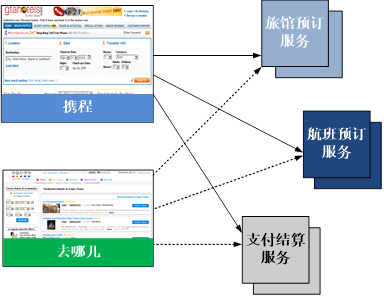
\includegraphics[scale=1]{fig/introduction/cloud_application_instance.png}
			\caption{云应用实例}
			\label{fig_cloud_application_instance}
			\centering\zihao{5}{Fig 1.1 Cloud application instance}
		\end{figure}

		云服务是以互联网为媒介面向用户按需提供的任何一种服务,它的表现形式多样但它的主要特点是能够动态满足用户提交的需求。云服务这一按需提供服务动态特性背后的基础是面向服务架构技术(service-oriented architecture,简写为SOA)。SOA技术在日益竞争激烈的市场环境中扮演着重要的角色,云服务提供商也是采取积极主动的态度大量采用该技术优化自身业务在云环境中的性能。举例来说图\ref{fig_cloud_application_instance}是两个云应用实例,集成了多个云服务包含了旅馆预订,航班预订以及支付结算服务。当用户面对如此功能相似几近相同的云服务,如何区分出这些云服务是用户当前面对的问题,也是学术界的热点。

		图 \ref{fig_The_cloud_architecture}是云服务市场架构示意图。在云环境中,云服务提供商掌握着大量的分布式资源像数据库,这类提供给开发人员设计云服务的资源和平台。当云应用务开发人员需要将多个云服务集成至云应用中,他们需要从云服务市场可用的云服务进行选择。同时这些云服务通常也都是动态地被来自全球各地且由不同通路连接调用进而集成至云应用中。调用云服务的用户往往都是处于不同的地理环境和网络环境。所以当他们在调用这些云服务的时候,连结至云服务的链路都是不同的,这也直接导致用户感受到的云服务质量是不同的。
		\begin{figure}[htb]
			\centering
			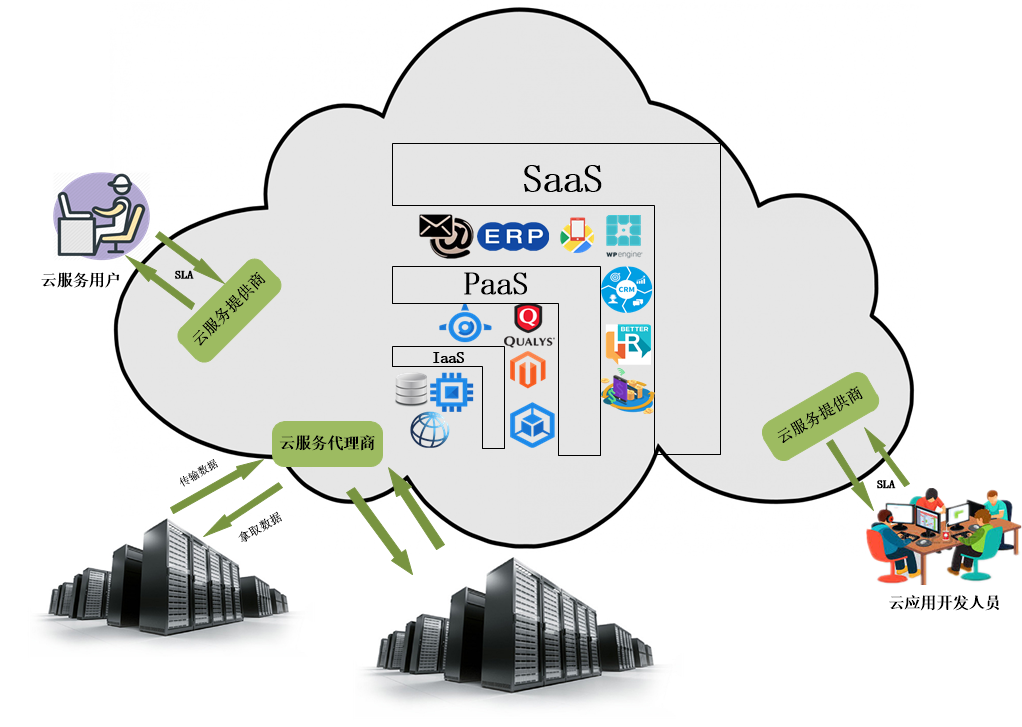
\includegraphics[scale=0.5]{fig/introduction/The_cloud_architecture.png}
			\caption{云市场结构}
			\label{fig_The_cloud_architecture}
			\centering\zihao{5}{Fig 1.2 The cloud architecture}
		\end{figure}
		
		服务质量(Quality of Service,简写为QoS)通常是用来刻画服务的非功能性特点。这也是云应用开发人员在进行云服务选择时十分关心的一个问题。进一步来说,将一些表现得低质的服务替换掉,用一些较好质量的服务取而代之能够整体提高云应用的表现和用户体验。     
		\subsection{研究意义}
		\label{subsec_meaning}
	\section{国内外研究现状}
	\label{sec_current_situation}
	\section{课题研究难点}
	\label{sec_main_points}
	\section{论文主要研究工作}
	\label{sec_main_works}
	\section{论文框架结构}
	\label{sec_paper_architecture}
	%这里是引言\upcite{MATSUMURA2017566,BHATTACHARYYA2010538}。
	\chapter{相关概念}
	\label{chapter_concepts}
	本章介绍论文中涉及到的相关概念及其背景知识,主要包含云服务中的QoS属性,云服务中的QoS预测问题,基于协同过滤的QoS预测方法,()。
	\section{云服务中的QoS属性}
	\label{sec_QoS_attributes}
	云计算近年来备受关注。云计算已经成为一个可扩展的服务消费和交付平台。云服务是云计算在用户端的表达,继承了云计算的特点。云服务不仅要满足用户的功能性需求外,还要满足QoS约束。
	
	服务质量(QoS)现已广泛运用在测量和评价系统或服务的非功能性特点的指标。QoS是可以从多个方面对系统或服务进行衡量,故具有多个属性指标,我们可以简单的归为两类。一类是用户相关属性,比如说价格(price),流行度(popularity)等;另一类是非用户相关属性,像响应时间(response-time),吞吐量(throughput)等。
	
	监测云服务QoS性能工作通常可以在云服务提供商一端进行,亦或也能在基于用户的角度进行观察。
	
		\subsection{响应时间(response-time)}
		\label{sec_response-time}
		响应时间是一项云服务去响应请求所花费的总时间也称为延迟时间(latency time),其中所主要构成包括网络往返时间(Network Round Trip Time,简写为Network RTT),重新传输时间(Retransmission Time,简写为Retrans),数据传输时间(Data Transfer Time,简写为Data Xfer)以及服务器响应时间(Server Response Time,简写为Server Resp)。所以,可以用公式 \ref{eq_compute_response-time}将QoS响应时间属性形式化表示。
		\begin{equation}
			response-time=NetworkRTT+Retrans+DataXfer+ServerResp
			\label{eq_compute_response-time}
		\end{equation}
		\subsection{吞吐量(Throughput)}
		\label{sec_throughput}
		吞吐量是指云服务在单位时间内成功处理请求事务的数量,是一个数学统计上的描述。由定义可知,公式 \ref{eq_compute_throughput}可以刻画这一属性。
		\begin{equation}
			throughput=\frac{\sum\limits_{i=0}^{t}Success(m,i)}{t_m}
			\label{eq_compute_throughput}
		\end{equation}
		\section{云服务中的QoS预测问题}
		\label{sec_QoS_Prediction_in_the_Cloud}
		\begin{figure}[htb]
			\centering
			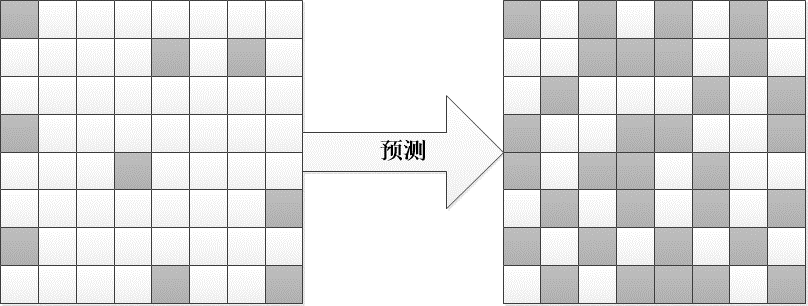
\includegraphics[scale=0.5]{fig/related_work/QoS_Prediction_Visualization.png}
			\caption{QoS预测问题形式化表达}
			\label{fig_QoS_Prediction_Visualization}
			\centering\zihao{5}{Fig 1.2 The cloud architecture}
		\end{figure}
		\section{基于协同过滤的QoS预测方法}
		\label{sec_QoS_Prediction_based_CF}
		
		\section{多目标(此处待定)}
		\label{sec_MultiObject}
	\chapter{创新点1}
	\label{chapter_novel_idea_1}
	这里是创新点1。
	\begin{figure}[htb]
		\centering 
			\subfigure[]{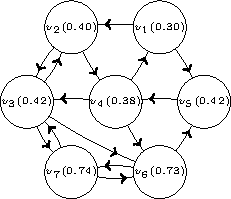
\includegraphics[scale=1]{fig/novel_idea_1/NG1.pdf}}
			\subfigure[]{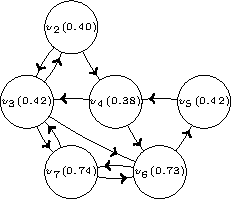
\includegraphics[scale=1]{fig/novel_idea_1/NG2.pdf}}
			\subfigure[]{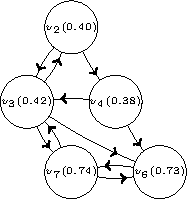
\includegraphics[scale=1]{fig/novel_idea_1/NG3.pdf}}
			\subfigure[]{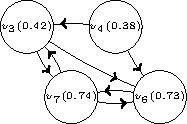
\includegraphics[scale=1]{fig/novel_idea_1/NG4.pdf}}
			\subfigure[]{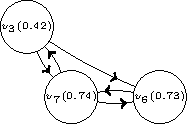
\includegraphics[scale=1]{fig/novel_idea_1/NG5.pdf}}
			\subfigure[]{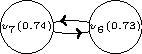
\includegraphics[scale=1]{fig/novel_idea_1/NG6.pdf}}
			\subfigure[]{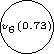
\includegraphics[scale=1]{fig/novel_idea_1/NG7.pdf}}
		\caption{NearestGraph算法实例转化图}
		\label{fig_QoS_distribution}
	\end{figure} 

	\begin{table}[htb]
		\caption{QoS数据集的数字特征}
		\label{table_Dataset_Statics}
		\centering
		\scalebox{0.85}[0.85]{
		\begin{tabular}{lll}
		\toprule  %添加表格头部粗线
		Statics &\quad Response-Time(seconds) &\quad Throughput(kbps)\\
		\hline
		Value Range &\qquad(0,20) &\qquad(0,1000)\\
		Mean &\qquad 0.910 &\qquad 47.386\\
		Median &\qquad 0.3320 &\qquad 11.07\\
		Standard Variance &\qquad 1.9320 &\qquad 107.4093\\
		User Num &\qquad 339 &\qquad 339\\
		Service Num &\qquad 5828 &\qquad 5828\\
		Records Num &\qquad 1974675 &\qquad 1974675\\
		\bottomrule %添加表格底部粗线
		\end{tabular}}
	\end{table}

	\begin{table}[htb]
		\centering
		\caption{性能对比}
		\label{table_Performance_Comparisons}
		\scalebox{0.7}[0.7]{
		\begin{tabular}{llllllll}
		\toprule
		Matrix &\multirow{2}*{Metrics\quad}&\multicolumn{6}{c}{Response-Time(seconds)}\\
		\cline{3-8}
		Density(\%)\qquad\quad& & UMean\qquad\qquad& IMean\qquad\qquad& UPCC\qquad\qquad& IPCC\qquad\qquad& WSRec\qquad\qquad& NearestGraph\\
		\multirow{2}*{10}& MAE& 0.8785& 0.7015& 0.6761& 0.6897& 0.6679& \textbf{0.6643}\\
		& RMSE& 1.8591& 1.5813& 1.4078& 1.4296& 1.4053& \textbf{1.4027}\\
		\multirow{2}*{20}& MAE& 0.8768& 0.6867& 0.5517& 0.5917& 0.5431& \textbf{0.5104}\\
		& RMSE& 1.8548& 1.5342& 1.3151& 1.3268& 1.2986& \textbf{1.2785}\\	
		\multirow{2}*{30}& MAE& 0.8747& 0.6818& 0.5159& 0.5037& 0.4927& \textbf{0.4723}\\
		& RMSE& 1.8557& 1.5311& 1.2680& 1.2252& 1.1973& \textbf{1.1246}\\
		\toprule
		Matrix&\multirow{2}*{Metrics\quad}&\multicolumn{6}{c}{Throughput(kbps)}\\
		\cline{3-8}
		Density(\%)\qquad\quad& & UMean\qquad\qquad& IMean\qquad\qquad& UPCC\qquad\qquad& IPCC\qquad\qquad& WSRec\qquad\qquad& NearestGraph\\
		\multirow{2}*{10}& MAE& 54.0084& 29.2651& 26.1230& 29.2651& 24.3285& \textbf{24.3269}\\
		& RMSE& 110.2821& 66.6334& 63.9573& 64.2285& 64.1908& \textbf{63.5435}\\
		\multirow{2}*{20}& MAE& 53.6768& 27.3393& 24.2695& 26.8318& 22.7717& \textbf{21.7493}\\
		& RMSE& 110.2977& 64.3986& 54.4783& 60.0825& 54.3701& \textbf{52.8731}\\	
		\multirow{2}*{30}& MAE& 53.8792& 26.6239& 23.7455& 26.4319& 21.3194& \textbf{19.6530}\\
		& RMSE& 110.1751& 64.3986& 54.4783& 57.8593& 51.7768& \textbf{50.5765}\\
		\bottomrule	
		\end{tabular}}
		\end{table}
	\chapter{创新点2}
	\label{chapter_novel_idea_2}
	这里是创新点2。
	\chapter{总结与展望}
	\label{chapter_summary_future}
	这里是总结与展望。
%%%%%%%%%%论文主体部分结束%%%%%%%%%%%%%%%%%%%%%%%%%	
	\nocite{*}
	\bibliography{ref/ref.bib}
	\begin{results}
	一、作者简历
	
	\quad 傅怡麒(1994-),男,江西省抚州市人,汉族
	
	\quad 教育背景:
	
	\quad 2012年9月-2016年7月\quad 沈阳师范大学软件学院 \quad 计算机科学与技术专业,获工学学士学位。
	
	\quad 2016年9月-2019年7月\quad 北京交通大学计算机信息与技术学院\quad 计算机科学与技术,攻读工学硕士学位。
	
	二、发表论文
	
	三、参与科研项目
\end{results}
	\begin{declaration}
	本人声明所呈交的学位论文是本人在导师指导下进行的研究工作和取得的研究成果,
	除了文中特别加以标注和致谢之处外,论文中不包含其他人已经发表或撰写过的研究成果,
	也不包含为获得北京交通大学或其他教育机构的学位或证书而使用过的材料。
	与我一同工作的同志对本研究所做的任何贡献均已在论文中作了明确的说明并表示了谢意。
	\\
	\\
	\\
	学位论文作者签名:\qquad\qquad\qquad\qquad\qquad 签字日期:\qquad\qquad 年\quad\quad 月\quad\quad 日
\end{declaration}
	\begin{metadata}
	\centering
	\begin{table}[htb]
		%\caption{数据集页} 
		\centering{\zihao{5}表1.1: 数据集页}
		\scalebox{0.85}[0.85]{ 
		\begin{tabular}{|l|l|l|l|l|}
			\hline
			关键词*\qquad\qquad\qquad & 密级*\qquad\qquad\qquad & 中图分类号\qquad\qquad & UDC\qquad\qquad\qquad\qquad & 论文资助\qquad\qquad \\
			\hline
			& & & & \\
			\hline
			\multicolumn{2}{|l|}{学位授予单位名称*} & 学位授予单位代码* & 学位类别* & 学位级别* \\
			\hline
			\multicolumn{2}{|l|}{北京交通大学} & 10004 &  &  \\
			\hline
			\multicolumn{2}{|l|}{论文题名} & \multicolumn{2}{|l|}{并列题名} &  论文语种* \\
			\hline
			\multicolumn{2}{|l|}{}&\multicolumn{2}{|l|}{}& \\
			\hline
			作者姓名* & \multicolumn{2}{l|}{} & 学号* & \\
			\hline
			\multicolumn{2}{|l|}{培养单位名称*} & 培养单位代码* & 培养单位地址 & 邮编 \\
			\hline
			\multicolumn{2}{|l|}{北京交通大学} & 10004 & 北京市海淀区 & 100044 \\
			\multicolumn{2}{|l|}{}& & 西直门外上园村3号 & \\
			\hline
			\multicolumn{2}{|l|}{学科专业*} & 研究方向* & 学制* & 学位授予年* \\
			\hline
			\multicolumn{2}{|l|}{} & & & \\
			\hline
			论文提交日期* & \multicolumn{4}{|l|}{} \\
			\hline
			导师姓名* & \multicolumn{2}{|l|}{} & 职称* & \\
			\hline
			评阅人 & \multicolumn{2}{|l|}{答辩委员会主席*} & \multicolumn{2}{|l|}{答辩委员会成员} \\
			& \multicolumn{2}{|l|}{} & \multicolumn{2}{|l|}{}  \\
			& \multicolumn{2}{|l|}{} & \multicolumn{2}{|l|}{} \\
			\hline
			\multicolumn{5}{|l|}{电子版论文提交格式  文本 (\quad)  图像 (\quad) 视频 (\quad) 音频 (\quad) 多媒体 (\quad) 其他 (\quad)}\\
			\multicolumn{5}{|l|}{推荐格式:application/msword;application/pdf} \\
			\hline
			\multicolumn{2}{|l|}{电子版论文出版(发布)者} & \multicolumn{2}{|l|}{电子版论文出版(发布)地} & 权限声明 \\
			\hline
			\multicolumn{2}{|l|}{} & \multicolumn{2}{|l|}{} & \\
			\hline
			论文总页数* & \multicolumn{4}{|l|}{} \\
			\hline
			\multicolumn{5}{|l|}{共33项,其中带*为必填数据,为21项。}\\
			\hline
		\end{tabular}
		}
	\end{table}
\end{metadata}
\end{document}